\documentclass[10pt, landscape, twocolumn]{article}

\usepackage[margin=0.5in, columnsep=0.4in]{geometry}
\usepackage{amsmath, amssymb, amsthm}
\usepackage{xcolor}
\usepackage{tabularx}
\usepackage{tikz}
\usetikzlibrary{arrows.meta, positioning, calc}
\usepackage{enumitem}
\usepackage{mathpazo} 
\usepackage{booktabs}
\usepackage{graphicx}

\pagestyle{empty} 
\setlength{\parindent}{0pt}
\setlength{\parskip}{4pt}

\AtBeginDocument{
  \setlength{\abovedisplayskip}{3pt}
  \setlength{\belowdisplayskip}{3pt}
  \setlength{\abovedisplayshortskip}{1pt}
  \setlength{\belowdisplayshortskip}{1pt}
}

\definecolor{themeblue}{RGB}{0, 90, 160}
\definecolor{themegray}{RGB}{80, 80, 80}

\newcommand{\cheatsheetsection}[1]{
    \vspace{0.6em}
    {\color{themeblue}\large\bfseries #1} \par
    \vspace{-0.5em}
    {\color{themeblue}\rule{\linewidth}{1pt}} \par
    \vspace{0.2em}
}

\newcommand{\cheatsheetsubsection}[1]{
    \vspace{0.4em}
    {\color{themeblue}\normalsize\bfseries #1} \par
    \vspace{0.1em}
}

\begin{document}

\begin{center}
    \vspace{-1em}
    {\color{themeblue}\huge\bfseries Linear Algebra Cheatsheet}\\[0.1em]
    {\color{themegray}\small Guide to Matrices, Subspaces, and Factorizations}\\[0.4em]
    {\color{themegray}\footnotesize \textbf{By Roberto León Landeros}}
\end{center}
\vspace{-1em}

\cheatsheetsection{1. Vectors, Matrices \& Spaces Fundamentals}
\textbf{Vector Space:} A set $V$ closed under addition and scalar multiplication satisfying 8 axioms: commutativity ($\mathbf{u}+\mathbf{v}=\mathbf{v}+\mathbf{u}$), associativity ($(\mathbf{u}+\mathbf{v})+\mathbf{w}=\mathbf{u}+(\mathbf{v}+\mathbf{w})$), zero vector ($\mathbf{v}+\mathbf{0}=\mathbf{v}$), additive inverse ($\mathbf{v}+(-\mathbf{v})=\mathbf{0}$), multiplicative identity ($1\mathbf{v}=\mathbf{v}$), distributivity of scalar sums ($(c+d)\mathbf{v}=c\mathbf{v}+d\mathbf{v}$), distributivity of vector sums ($c(\mathbf{u}+\mathbf{v})=c\mathbf{u}+c\mathbf{v}$), and scalar associativity ($c(d\mathbf{v})=(cd)\mathbf{v}$).\\
\textbf{Basic Operations:} For $\mathbf{u} = (u_1, u_2, \dots, u_n)$ and $\mathbf{v} = (v_1, v_2, \dots, v_n)$:
\begin{itemize}[leftmargin=*, itemsep=4pt, parsep=0pt]
    \item Addition: $\mathbf{u} + \mathbf{v} = (u_1+v_1, u_2+v_2, \dots, u_n+v_n)$
    \item Scalar Multiplication: $c\mathbf{u} = (cu_1, cu_2, \dots, cu_n)$
    \item Cross Product ($\mathbb{R}^3$): $\mathbf{u} \times \mathbf{v} = \det \left[ \begin{smallmatrix} \hat{\mathbf{i}} & \hat{\mathbf{j}} & \hat{\mathbf{k}} \\ u_1 & u_2 & u_3 \\ v_1 & v_2 & v_3 \end{smallmatrix} \right] \\= (u_2v_3 - u_3v_2)\hat{\mathbf{i}} - (u_1v_3 - u_3v_1)\hat{\mathbf{j}} + (u_1v_2 - u_2v_1)\hat{\mathbf{k}}$
    \item Norm (Length): $\|\mathbf{u}\| = \sqrt{\mathbf{u} \cdot \mathbf{u}}$
\end{itemize}
\textbf{Geometry \& Inequalities:} Cauchy-Schwarz: $|\mathbf{u} \cdot \mathbf{v}| \leq \|\mathbf{u}\|\|\mathbf{v}\|$. Triangle Inequality: $\|\mathbf{u} + \mathbf{v}\| \leq \|\mathbf{u}\| + \|\mathbf{v}\|$. Angle between vectors: $\cos\theta = \frac{\mathbf{u} \cdot \mathbf{v}}{\|\mathbf{u}\|\|\mathbf{v}\|}$.\\
\textbf{Dependence \& Basis:} Linearly Independent if $c_1\mathbf{v}_1 + \dots + c_n\mathbf{v}_n = 0 \implies c_i = 0$ for all $i$. A basis is a linearly independent set that spans the space. \\For subspaces $A$ and $B$, the dimension formula is $\dim(A+B) = \dim(A) + \dim(B) - \dim(A \cap B)$.\\
Let $\mathbf{u}, \mathbf{v} \in \mathbb{R}^n$. The dot product is $\mathbf{u} \cdot \mathbf{v} = \mathbf{u}^T \mathbf{v} = \sum u_i v_i = \|\mathbf{u}\|\|\mathbf{v}\|\cos\theta$.\\
Orthogonality: $\mathbf{u} \perp \mathbf{v} \iff \mathbf{u} \cdot \mathbf{v} = 0$.
A matrix $A \in \mathbb{R}^{m \times n}$ represents a linear transformation $T: \mathbb{R}^n \to \mathbb{R}^m$. \\
The identity matrix $I$ acts as the multiplicative unit ($AI = IA = A$); $I = \left[ \begin{smallmatrix} 1 & 0 & 0 \\ 0 & 1 & 0 \\ 0 & 0 & 1 \end{smallmatrix} \right]$.

\cheatsheetsection{2. Views of Matrix Multiplication}
Let $A \in \mathbb{R}^{m \times n}$ and $B \in \mathbb{R}^{n \times p}$. The product $C = AB$ is an $m \times p$ matrix.
\begin{itemize}[leftmargin=*, itemsep=2pt, parsep=0pt]
    \item \textbf{1. Standard (Dot Product):} $c_{ij} = \displaystyle\sum\limits_{k=1}^n a_{ik}b_{kj} = (\text{row } i \text{ of } A) \cdot (\text{col } j \text{ of } B)$.
    \item \textbf{2. Column View (Linear Combination of Columns):} The columns of $C$ are combinations of the columns of $A$. 
    \[ AB = A \begin{bmatrix} | & & | \\ \mathbf{b}_1 & \dots & \mathbf{b}_p \\ | & & | \end{bmatrix} = \begin{bmatrix} | & & | \\ A\mathbf{b}_1 & \dots & A\mathbf{b}_p \\ | & & | \end{bmatrix} \]
    \item \textbf{3. Row View (Linear Combination of Rows):} The rows of $C$ are combinations of the rows of $B$.
    \[ AB = \begin{bmatrix} - & \mathbf{a}_1 & - \\ & \vdots & \\ - & \mathbf{a}_m & - \end{bmatrix} B = \begin{bmatrix} - & \mathbf{a}_1 B & - \\ & \vdots & \\ - & \mathbf{a}_m B & - \end{bmatrix} \]
    \item \textbf{4. Outer Product (Sum of Rank-1 Matrices):} $AB$ is the sum of columns of $A$ times rows of $B$.
    \[ AB = \sum_{k=1}^n (\text{col } k \text{ of } A)(\text{row } k \text{ of } B) = \sum_{k=1}^n \mathbf{a}_k \mathbf{b}_k^T \]
    \item \textbf{5. Block Matrices (Submatrices):} Matrices can be multiplied as scalars if blocks are compatible.
    \[ \begin{bmatrix} A & B \\ C & D \end{bmatrix} \begin{bmatrix} E & F \\ G & H \end{bmatrix} = \begin{bmatrix} AE+BG & AF+BH \\ CE+DG & CF+DH \end{bmatrix} \]
\end{itemize}

\cheatsheetsection{3. The Four Fundamental Subspaces}
Let $A \in \mathbb{R}^{m \times n}$ have rank $r$ (number of pivots). The Fundamental Theorem of Linear Algebra states:

\begin{tabularx}{\linewidth}{p{0.3\linewidth}p{0.25\linewidth}X}
\toprule
\textbf{Subspace} & \textbf{Dim} & \textbf{Basis \& Location} \\ \midrule
$\operatorname{Col}(A)$ (Column Space) & $r$ & Pivot columns of $A$. Lives in $\mathbb{R}^m$. \\ 
$\operatorname{Null}(A)$ (Nullspace) & $n - r$ & Special solutions to $Ax=0$. Lives in $\mathbb{R}^n$. \\ 
$\operatorname{Row}(A) = \operatorname{Col}(A^T)$ & $r$ & Non-zero rows of RREF. Lives in $\mathbb{R}^n$. \\ 
$\operatorname{Null}(A^T)$ (Left Nullspace) & $m - r$ & Solutions to $A^T y = 0$. Lives in $\mathbb{R}^m$. \\ \bottomrule
\end{tabularx}

\textbf{Orthogonality:} $\operatorname{Row}(A) \perp \operatorname{Null}(A)$ in $\mathbb{R}^n$ and $\operatorname{Col}(A) \perp \operatorname{Null}(A^T)$ in $\mathbb{R}^m$. Any $x \in \mathbb{R}^n$ can be split into $x = x_r + x_n$.

\vspace{0.1em}
\begin{center}
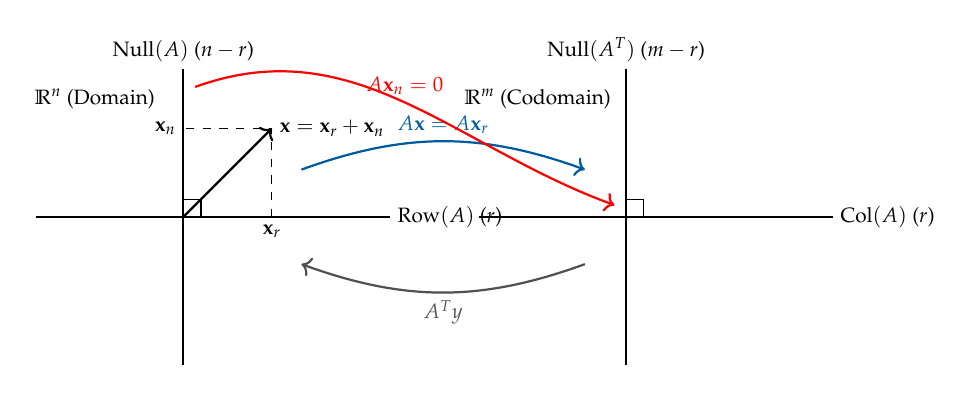
\begin{tikzpicture}[scale=0.75, transform shape]
    \draw[thick] (-2.5,0) -- (3.5,0) node[right] {$\operatorname{Row}(A)$ ($r$)};
    \draw[thick] (0,-2.5) -- (0,2.5) node[above] {$\operatorname{Null}(A)$ ($n-r$)};
    \node at (-1.5, 2) {$\mathbb{R}^n$ (Domain)};
    \draw (0.3,0) -- (0.3,0.3) -- (0,0.3);
    \draw[->, thick] (0,0) -- (1.5,1.5) node[right] {$\mathbf{x} = \mathbf{x}_r + \mathbf{x}_n$};
    \draw[dashed] (1.5,0) -- (1.5,1.5) -- (0,1.5);
    \node[below] at (1.5,0) {$\mathbf{x}_r$};
    \node[left] at (0,1.5) {$\mathbf{x}_n$};

    \begin{scope}[xshift=7.5cm]
        \draw[thick] (-2.5,0) -- (3.5,0) node[right] {$\operatorname{Col}(A)$ ($r$)};
        \draw[thick] (0,-2.5) -- (0,2.5) node[above] {$\operatorname{Null}(A^T)$ ($m-r$)};
        \node at (-1.5, 2) {$\mathbb{R}^m$ (Codomain)};
        \draw (0.3,0) -- (0.3,0.3) -- (0,0.3);
    \end{scope}

    \draw[->, thick, themeblue] (2, 0.8) to[out=20,in=160] node[above] {$A\mathbf{x} = A\mathbf{x}_r$} (6.8, 0.8);
    \draw[->, thick, red] (0.2, 2.2) to[out=20,in=160] node[above] {$A\mathbf{x}_n = 0$} (7.3, 0.2);
    \draw[->, thick, themegray] (6.8, -0.8) to[out=200,in=-20] node[below] {$A^T y$} (2, -0.8);
\end{tikzpicture}
\end{center}

\cheatsheetsection{4. Systems of Equations \& Elimination}
To solve $Ax = b$, we construct $[A \mid b]$ and apply row operations to reach Reduced Row Echelon Form (RREF).
\begin{itemize}[leftmargin=*, itemsep=4pt, parsep=0pt]
    \item \textbf{Elementary Matrices ($E$):} Left-multiply to perform row operations. E.g., subtract $l_{21}$ times row 1 from row 2:
    \[ E_{21} = \begin{bmatrix} 1 & 0 & 0 \\ -l_{21} & 1 & 0 \\ 0 & 0 & 1 \end{bmatrix}, \quad E_{21}A = \begin{bmatrix} \text{row } 1 \\ \text{row } 2 - l_{21}(\text{row } 1) \\ \text{row } 3 \end{bmatrix} \]
    \item \textbf{Permutation Matrices ($P$):} Reorder rows (left-multiply) or columns (right-multiply). $P^{-1} = P^T$.
    \item \textbf{Existence \& Uniqueness:} $Ax=b$ has a solution $\iff b \in \operatorname{Col}(A)$. Unique solution $\iff \operatorname{Null}(A) = \{0\}$ (full column rank, $r=n$).
    \item \textbf{Left/Right Inverses:} If $r=n$ (full column rank), $A$ has a Left Inverse: $A_{left}^{-1} = (A^T A)^{-1}A^T$. If $r=m$ (full row rank), $A$ has a Right Inverse: $A_{right}^{-1} = A^T(AA^T)^{-1}$.
    \item \textbf{Rouché-Frobenius Theorem:} No solution if $\operatorname{rank}(A) < \operatorname{rank}([A \mid b])$. Unique solution if $\operatorname{rank}(A) = \operatorname{rank}([A \mid b]) = n$. Infinite solutions if $\operatorname{rank}(A) = \operatorname{rank}([A \mid b]) < n$.
\end{itemize}

\cheatsheetsection{5. Determinants \& Inverses}
The determinant $\det(A)$ or $|A|$ is only defined for square $n \times n$ matrices. Geometrically, it measures the scaling factor of the linear transformation (Area in $\mathbb{R}^2$, Volume in $\mathbb{R}^3$ of the parallelepiped formed by the columns).
\begin{itemize}[leftmargin=*, itemsep=4pt, parsep=0pt]
    \item \textbf{Properties:}
    $\begin{aligned}[t]
        \det(AB) &= \det(A)\det(B) \\
        \det(A^T) &= \det(A) \\
        \det(A^{-1}) &= 1/\det(A) \\
        \det(cA) &= c^n\det(A) \\
        \det(A+B) &\neq \det(A)+\det(B) \text{ (generally)}
    \end{aligned}$
    \item Row exchange flips sign. Multiplying a row by $c$ scales det by $c$. Adding a multiple of one row to another does not change the determinant.
    \item Determinant of a triangular matrix is the product of its diagonal entries.
    \item $\det(A) \neq 0 \iff A$ is invertible $\iff \operatorname{Null}(A) = \{0\}$.
    \item \textbf{Laplace Expansion (Cofactors):} $\det(A) = \sum_{j=1}^n a_{ij}C_{ij}$, where $C_{ij} = (-1)^{i+j}\det(M_{ij})$.
    \\
    \item \textbf{Leibniz Formula:} $\det(A) = \sum_{\sigma \in S_n} \operatorname{sgn}(\sigma) \prod_{i=1}^n a_{i,\sigma(i)}$, where $\sigma$ are permutations and $\operatorname{sgn}$ is the parity.
    \item \textbf{Practical Inverse (Adjugate):} $A^{-1} = \frac{1}{\det(A)} C^T$.
    \item \textbf{Block Matrices Inverse:} If $A, D$ are invertible:
    $\left[ \begin{smallmatrix} A & 0 \\ 0 & D \end{smallmatrix} \right]^{-1} = \left[ \begin{smallmatrix} A^{-1} & 0 \\ 0 & D^{-1} \end{smallmatrix} \right]$
    \item \textbf{Cramer's Rule:} To solve $Ax=b$, $x_i = \frac{\det(A_i)}{\det(A)}$, where $A_i$ is $A$ with its $i$-th column replaced by $b$.
\end{itemize}

\cheatsheetsection{6. Factorizations: The Big Picture}
Decomposing a matrix reveals its fundamental structure and simplifies complex operations. 

\cheatsheetsubsection{A. LU Decomposition (Elimination)}
$A = LU$. Separates $A$ into a lower triangular $L$ (multipliers) and upper triangular $U$ (pivots). If row swaps are needed, $PA = LU$.

\cheatsheetsubsection{B. QR Decomposition (Gram-Schmidt)}
$A = QR$. $Q$ has orthonormal columns ($Q^T Q = I$), $R$ is upper triangular. Used for stable least squares and eigenvalue algorithms. Iterative orthogonal projection: $\mathbf{u}_k = \mathbf{a}_k - \sum_{i=1}^{k-1} \operatorname{proj}_{\mathbf{u}_i}(\mathbf{a}_k)$.

\cheatsheetsubsection{C. Eigen-Decomposition (Diagonalization)}
$A = X \Lambda X^{-1}$. $X$ contains eigenvectors as columns, $\Lambda$ has eigenvalues on the diagonal. Requires $n$ independent eigenvectors.
\[ A = \begin{bmatrix} | & & | \\ \mathbf{x}_1 & \dots & \mathbf{x}_n \\ | & & | \end{bmatrix} \begin{bmatrix} \lambda_1 & & \\ & \ddots & \\ & & \lambda_n \end{bmatrix} X^{-1} \]

\cheatsheetsubsection{D. Spectral Theorem (Symmetric Matrices)}
If $A = A^T$, eigenvalues are real, and eigenvectors are orthogonal. $A = Q \Lambda Q^T$, where $Q$ is an orthogonal matrix. 

\cheatsheetsubsection{E. Singular Value Decomposition (SVD)}
The crown jewel. Exists for ANY $m \times n$ matrix. $A = U \Sigma V^T$.
\begin{itemize}[leftmargin=*, itemsep=4pt, parsep=0pt]
    \item $U \in \mathbb{R}^{m \times m}$ (Orthogonal, left singular vectors, basis for $\operatorname{Col}(A), \operatorname{Null}(A^T)$).
    \item $V \in \mathbb{R}^{n \times n}$ (Orthogonal, right singular vectors, basis for $\operatorname{Row}(A), \operatorname{Null}(A)$).
    \item $\Sigma \in \mathbb{R}^{m \times n}$ (Diagonal, singular values $\sigma_i = \sqrt{\lambda_i(A^T A)}$).
    \item \textbf{Pseudoinverse:} The Moore-Penrose pseudoinverse is $A^+ = V \Sigma^+ U^T$.
\end{itemize}

\cheatsheetsection{7. Eigenvalues \& Eigenvectors}
$\mathbf{x}$ is an eigenvector of $A$ if $A\mathbf{x} = \lambda \mathbf{x}$. The action of the matrix simplifies to a scalar multiplication.
\begin{itemize}[leftmargin=*, itemsep=4pt, parsep=0pt]
    \item \textbf{Characteristic Equation:} $\det(A - \lambda I) = 0$. Roots are $\lambda_i$.
    \item \textbf{Nullspace Link:} Eigenvectors are the basis of $\operatorname{Null}(A - \lambda I)$.
    \item \textbf{Multiplicity \& Diagonalization:} $A$ is diagonalizable $\iff$ algebraic multiplicity equals geometric multiplicity ($\dim(\operatorname{Null}(A - \lambda I))$) for all eigenvalues.
    \item \textbf{Trace \& Det:} $\sum \lambda_i = \operatorname{tr}(A)$ and $\prod \lambda_i = \det(A)$.
    \item \textbf{Powers:} $A^k = X \Lambda^k X^{-1}$. $A^k \mathbf{x} \to 0$ if all $|\lambda_i| < 1$.
    \item \textbf{Markov Matrices:} Columns sum to 1. Always has $\lambda = 1$. The corresponding eigenvector is the steady state.
\end{itemize}

\cheatsheetsection{8. Orthogonality \& Projections}
A matrix $Q$ with orthonormal columns satisfies $Q^T Q = I$. If $Q$ is square, $Q^T = Q^{-1}$. Multiplication by $Q$ preserves lengths: $\|Q\mathbf{x}\| = \|\mathbf{x}\|$.

\cheatsheetsubsection{Projections}
To project a vector $\mathbf{b}$ onto $\operatorname{Col}(A)$, the error $\mathbf{e} = \mathbf{b} - \mathbf{p}$ must be orthogonal to $\operatorname{Col}(A)$, meaning $A^T(\mathbf{b} - A\hat{\mathbf{x}}) = 0$.
\begin{itemize}[leftmargin=*, itemsep=4pt, parsep=0pt]
    \item \textbf{Normal Equations:} $A^T A \hat{\mathbf{x}} = A^T \mathbf{b}$.
    \item \textbf{Projection Matrix:} $P = A(A^T A)^{-1}A^T$. Properties: $P^2 = P$ and $P^T = P$.
    \item \textbf{1D Projection:} Onto a line $\mathbf{a}$: $P = \frac{\mathbf{a}\mathbf{a}^T}{\mathbf{a}^T \mathbf{a}}$.
\end{itemize}

\cheatsheetsection{9. Linear Transformations}
A linear transformation $T(\mathbf{x}) = A\mathbf{x}$ obeys $T(c\mathbf{x} + \mathbf{y}) = cT(\mathbf{x}) + T(\mathbf{y})$.
\begin{itemize}[leftmargin=*, itemsep=4pt, parsep=0pt]
    \item \textbf{Matrix Representation:} The $j$-th column of $A$ is $T(\mathbf{e}_j)$.
    \item \textbf{Rotation:} Counterclockwise by $\theta$:
    $R_\theta = \left[ \begin{smallmatrix} \cos\theta & -\sin\theta \\ \sin\theta & \cos\theta \end{smallmatrix} \right]$
    \item \textbf{Change of Basis \& Similar Matrices:} If $B$ is the matrix of basis vectors, a vector $\mathbf{v}$ in standard basis relates to coordinates $\mathbf{c}$ in $B$-basis by $\mathbf{v} = B\mathbf{c}$. Similar matrices represent the same transformation in different bases: $M = B^{-1} A B$. They share the same eigenvalues, trace, and determinant.
    \item \textbf{Rank-Nullity Theorem:} For a linear transformation $T: V \to W$, $\dim(V) = \operatorname{rank}(T) + \operatorname{nullity}(T)$.
\end{itemize}

\cheatsheetsection{10. Special Matrices Summary}
\begin{itemize}[leftmargin=*, itemsep=4pt, parsep=0pt]
    \item \textbf{Symmetric:} $A = A^T$. Real eigenvalues, orthogonal eigenvectors.
    \item \textbf{Positive Definite:} $A = A^T$ and $\mathbf{x}^T A \mathbf{x} > 0$ for all $\mathbf{x} \neq 0$. All $\lambda_i > 0$. All pivots $> 0$. $A = R^T R$ (Cholesky). \textbf{Sylvester's Criterion:} All leading principal minors have positive determinants ($\det > 0$).
    \item \textbf{Orthogonal:} $Q^T Q = I$. Columns form an orthonormal basis. $\det(Q) = \pm 1$. Eigenvalues $|\lambda| = 1$.
    \item \textbf{Rank-1:} $A = \mathbf{u}\mathbf{v}^T$. $\operatorname{Col}(A)$ is the line through $\mathbf{u}$. $\operatorname{Row}(A)$ is the line through $\mathbf{v}$. Has $\lambda = \mathbf{v}^T \mathbf{u}$ and $n-1$ zero eigenvalues.
    \item \textbf{Skew-Symmetric:} $A = -A^T$. Pure imaginary eigenvalues.
    \item \textbf{Idempotent:} $P^2 = P$. Typical of projection matrices.
    \item \textbf{Nilpotent:} $A^k = 0$ for some integer $k$.
\end{itemize}

\cheatsheetsection{11. Quadratic Forms \& Matrix Exponentials}
\begin{itemize}[leftmargin=*, itemsep=4pt, parsep=0pt]
    \item \textbf{Quadratic Forms:} Expressed as $f(\mathbf{x}) = \mathbf{x}^T A \mathbf{x}$ for a symmetric matrix $A$. The Hessian matrix contains second partial derivatives, critical for multivariable optimization.
    \item \textbf{Matrix Exponential ($e^{At}$):} $e^{At} = I + At + \frac{1}{2!}(At)^2 + \dots = \sum_{k=0}^{\infty} \frac{(At)^k}{k!}$. Used to solve linear systems of differential equations $\frac{d\mathbf{u}}{dt} = A\mathbf{u}$, with solution $\mathbf{u}(t) = e^{At}\mathbf{u}(0)$.
\end{itemize}

\newpage
\cheatsheetsection{12. Mini-Algorithms (Pipelines)}
\begin{itemize}[leftmargin=*, itemsep=4pt, parsep=0pt]
    \item \textbf{Solve $Ax = b$:} $[A \mid b] \xrightarrow{\text{RREF}} \text{Check pivots:} \begin{cases} \text{Row } [0\dots0 \mid c\neq0] \implies \text{\textbf{No Solution}} \\ r = n \implies \text{\textbf{Unique}} \\ r < n \implies \boldsymbol{\infty} \text{ \textbf{Solutions (Free Vars)}} \end{cases}$
    \item \textbf{Subspace Bases:} $A \xrightarrow{\text{RREF}} \implies \begin{cases} \operatorname{Col}(A): \text{Original cols of } A \text{ at pivot positions} \\ \operatorname{Null}(A): \text{Set one free var}=1 \text{ (others } 0) \to \text{Solve} \end{cases}$
    \item \textbf{Rank ($r$):} $A \xrightarrow{\text{Echelon Form}} \implies r = \text{Total number of pivots}$
    \item \textbf{Eigenvalues \& Vectors:} $\det(A-\lambda I)=0 \xrightarrow{\text{Roots}} \lambda_i \implies \text{Find basis for } \operatorname{Null}(A-\lambda_i I) \xrightarrow{\text{Yields}} \mathbf{x}_i$
    \item \textbf{Diagonalization ($A=X\Lambda X^{-1}$):} Find $n$ independent $\mathbf{x}_i \implies X = [\mathbf{x}_1 \dots \mathbf{x}_n] \implies \Lambda = \operatorname{diag}(\lambda_1 \dots \lambda_n)$
    \item \textbf{Gram-Schmidt:} $\mathbf{u}_1 = \mathbf{a}_1 \implies \mathbf{u}_k = \mathbf{a}_k - \sum \operatorname{proj}_{\mathbf{u}_j}(\mathbf{a}_k) \implies \text{Normalize: } \mathbf{q}_k = \frac{\mathbf{u}_k}{\|\mathbf{u}_k\|}$
    \item \textbf{Least Squares ($\hat{x}$):} $Ax=b \text{ (inconsistent)} \xrightarrow{\text{Left-mult } A^T} A^TA\hat{\mathbf{x}} = A^T\mathbf{b} \implies \text{Solve for } \hat{\mathbf{x}}$
\end{itemize}

\cheatsheetsection{13. The Big Picture (Concept Graphs)}
\begin{itemize}[leftmargin=*, itemsep=4pt, parsep=0pt]
    \item \textbf{LU} $\implies$ Gaussian Elimination $\implies$ Solves $Ax=b$ efficiently for multiple $\mathbf{b}$'s
    \item \textbf{QR} $\implies$ Orthogonality $\implies$ Projections $\implies$ Stable Least Squares ($R\hat{\mathbf{x}} = Q^T\mathbf{b}$)
    \item \textbf{SVD} $\implies$ Rotations + Scaling ($U\Sigma V^T$) $\implies$ Full Structure $\implies$ Defines 4 Fundamental Subspaces
    \item \textbf{Eigen} $\implies$ Diagonalization ($A=X\Lambda X^{-1}$) $\implies$ Decouples Variables $\implies$ Dynamics \& Powers ($A^k$)
\end{itemize}

\cheatsheetsection{14. 
Common Pitfalls ($\neq$)}
\begin{itemize}[leftmargin=*, itemsep=4pt, parsep=0pt]
    \item $\mathbf{AB \neq BA} \implies$ Matrix multiplication is \textbf{not commutative}. Order is strict.
    \item $\mathbf{\det(A+B) \neq \det(A) + \det(B)} \implies$ Determinant is entirely non-linear over addition.
    \item \textbf{Independence} $\mathbf{\nRightarrow}$ \textbf{Orthogonality} $\implies$ Orthogonal vectors are independent, but not vice versa.
    \item \textbf{Invertible} $\mathbf{\nLeftrightarrow}$ \textbf{Diagonalizable} $\implies$ Totally unrelated properties (e.g., $\left[\begin{smallmatrix}1&1\\0&1\end{smallmatrix}\right]$ invertible but not diag).
    \item \textbf{Order Reversal} $\implies$ Transposes \& inverses flip order: $(AB)^T = B^T A^T$ and $(AB)^{-1} = B^{-1} A^{-1}$.
    \item \textbf{Projection Trap} $\implies$ For $P = A(A^TA)^{-1}A^T$, you \textbf{cannot} distribute the inverse unless $A$ is square.
\end{itemize}

\cheatsheetsection{15. Key Intuitions ($\to$)}
\begin{itemize}[leftmargin=*, itemsep=4pt, parsep=0pt]
    \item \textbf{Determinant} $\to$ Volume scaling factor. ($\det=0 \implies$ space collapses, information is lost).
    \item \textbf{Eigenvalues} $\to$ Stretch/shrink factors along invariant directions.
    \item \textbf{Rank} $\to$ True dimensionality (information content) of the output space.
    \item \textbf{Nullspace} $\to$ Invisibility. Inputs that get crushed to the zero vector.
    \item \textbf{Projections} $\to$ Closest "shadow" in a subspace. Error vector is strictly $\perp$ to the subspace.
\end{itemize}

\cheatsheetsection{16. Exam Tips \& Verifications}
\begin{itemize}[leftmargin=*, itemsep=4pt, parsep=0pt]
    \item \textbf{Check Eigenvalues:} Always verify $\sum \lambda_i = \operatorname{tr}(A)$ (diagonal sum) and $\prod \lambda_i = \det(A)$.
    \item \textbf{Symmetric Shortcut:} $A = A^T \implies$ Always diagonalizable, real $\lambda$'s, orthogonal eigenvectors.
    \item \textbf{Orthogonal Shortcut:} $Q^T Q = I \implies Q^{-1} = Q^T$ (Zero calculation required for inverse).
    \item \textbf{Zero Eigenvalue:} $\lambda=0 \implies \det(A)=0 \implies$ Singular $\implies \operatorname{Null}(A)$ contains non-zero vectors.
    \item \textbf{Dependence Spotting:} Proportional rows/cols or all-zero row $\implies \det=0$ and $r<n$.
\end{itemize}
\end{document}